% !TEX program = pdflatex
% Projeto Individual 1 -- PPMEC0070 / Redes Neurais e Aprendizado Profundo (2026/2)
% Universidade de Brasilia -- Prof. Dibio Leandro Borges
%
% Primeira versao do artigo em formato IEEE (dupla coluna), gerada a partir dos
% resultados reais documentados em Projeto-1/resultados {1,2,3,4}/.
% Nenhum numero neste arquivo foi inventado -- todos vem dos logs/CSVs de treino reais.

\documentclass[conference]{IEEEtran}
\IEEEoverridecommandlockouts

\usepackage{cite}
\usepackage{amsmath}
\usepackage{amssymb}
\usepackage{graphicx}
\usepackage{booktabs}
\usepackage{url}
\usepackage[utf8]{inputenc}
\usepackage[T1]{fontenc}
\usepackage[hidelinks]{hyperref}

\def\BibTeX{{\rm B\kern-.05em{\sc i\kern-.025em b}\kern-.08em
    T\kern-.1667em\lower.7ex\hbox{E}\kern-.125emX}}

\begin{document}

\title{MachadoGPT: Corpus, Resultados e Busca Automatizada de Hiperparâmetros}

\author{
\IEEEauthorblockN{Ronen Rodrigues Silva Filho}
\IEEEauthorblockA{
Programa de Pós-Graduação em Sistemas Mecatrônicos (PPMEC)\\
Universidade de Brasília (UnB)\\
Matrícula: 262122402 \\
ronen.filho@gmail.com \\[4pt]
\textit{Projeto Individual 1 -- PPMEC0070 - Cibernética e Aprendizagem de Máquinas, 2026/2}\\
\textit{Prof.\ Dibio Leandro Borges}}
}

\maketitle

\begin{abstract}
This work implements, trains, and evaluates a character-level autoregressive
language model in the style of GPT-2, trained exclusively on the works of
Machado de Assis, using Andrej Karpathy's \textit{nanoGPT} as the mandatory
base code, as required by the assignment for Individual Project 1 of the
Cybernetics and Machine Learning course (PPMEC0070/UnB). We built a custom
corpus of 13,978,947 characters (2,392,278 words) by combining the 12 works
by Machado available on Project Gutenberg with 1,781 pages extracted from
the Portuguese Wikisource via a recursive category crawl -- about 3.5 times
larger than the first version of the corpus and larger than the equivalent
public datasets found. Three controlled training runs isolate the effect of
corpus size and training budget: the best validated result reaches a
\textit{val loss} of 1.1040 (perplexity $\approx 3.02$) after 15,000
iterations, with no signs of \textit{overfitting}, surpassing nanoGPT's
official baseline (\textit{shakespeare\_char}, 1.4697) and our own two
earlier runs. We then built an automated search infrastructure (book-level
\textit{k-fold} cross-validation, \textit{successive halving}) to test three
axes of improvement -- architecture/hyperparameters, positional embedding
strategy, and tokenization -- which points to promising candidates under a
reduced budget, but whose confirmation under the full training budget fails
systematically (numerical divergence), a genuine methodological finding
about the limits of mixed-precision training on Apple's MPS backend, which
we diagnose and document. Finally, we discuss how the project could be
extended to answer questions within the Machado de Assis universe,
proposing a retrieval-augmented generation (RAG) approach over the corpus
itself.
\end{abstract}

\begin{IEEEkeywords}
language models, transformers, GPT-2, nanoGPT, natural language processing,
Machado de Assis, text generation
\end{IEEEkeywords}

\vspace{6pt}
\noindent{\small\bfseries\itshape Resumo---}{\small Este trabalho implementa,
treina e avalia um modelo de linguagem autorregressivo em nível de
caractere, no estilo GPT-2, treinado exclusivamente na obra de Machado de
Assis, usando o \textit{nanoGPT} de Andrej Karpathy como código base,
conforme exigido pelo enunciado do Projeto Individual 1 da disciplina
Cibernética e Aprendizagem de Máquinas (PPMEC0070/UnB). Foi construído um
corpus próprio de 13.978.947 caracteres (2.392.278 palavras), combinando as
12 obras de Machado disponíveis no Project Gutenberg com 1.781 páginas
extraídas do Wikisource em português via crawl recursivo de categoria --
cerca de 3,5 vezes maior que a primeira versão do corpus e maior que os
datasets públicos equivalentes encontrados. Três rodadas de treino
controladas isolam o efeito do tamanho do corpus e do orçamento de
iterações: o melhor resultado validado atinge \textit{val loss} de 1,1040
(perplexidade $\approx 3{,}02$) em 15.000 iterações, sem sinais de
\textit{overfitting}, superando o baseline oficial do nanoGPT
(\textit{shakespeare\_char}, 1,4697) e as duas rodadas anteriores próprias.
Em seguida, foi construída uma infraestrutura de busca automatizada
(validação cruzada \textit{k-fold} por obra, \textit{successive halving})
para testar três eixos de melhoria -- arquitetura/hiperparâmetros,
estratégia de \textit{embedding} posicional e tokenização -- que aponta
candidatos promissores em orçamento reduzido, mas cuja confirmação em
orçamento completo falha de forma sistemática (divergência numérica), um
achado metodológico genuíno sobre os limites do treinamento em precisão
mista no backend MPS da Apple, diagnosticado e documentado. Por fim, é
discutido como o projeto poderia ser estendido para responder perguntas no
universo machadiano, propondo-se uma abordagem de recuperação aumentada por
geração (RAG) sobre o próprio corpus.}

\vspace{4pt}
\noindent{\small\bfseries\itshape Palavras-chave---}{\small modelos de
linguagem, transformers, GPT-2, nanoGPT, processamento de linguagem
natural, Machado de Assis, geração de texto}

\vspace{6pt}

\section{Introdução}

O enunciado do Projeto Individual 1 pede a implementação, o treinamento e a
avaliação de um modelo de linguagem semelhante ao GPT-2 \cite{radford2019gpt2},
treinado com o conteúdo das obras de Machado de Assis, usando o
\textit{nanoGPT} \cite{karpathy_nanogpt} como código base obrigatório. Machado
de Assis é um domínio de texto particularmente interessante para esse
exercício: sua obra é de domínio público, estilisticamente reconhecível (uso
de travessão para diálogo, mistura de ortografia de época, ironia narrativa),
e grande o suficiente -- se agregada de mais de uma fonte -- para sustentar o
treinamento de um modelo do zero, sem depender de \textit{pretraining} externo.

Este artigo documenta cinco contribuições concretas:
\begin{enumerate}
  \item um \emph{pipeline} próprio e reprodutível de construção de corpus que
        combina duas fontes de domínio público (Seção~\ref{sec:corpus}),
        resultando em um corpus consideravelmente maior que alternativas
        públicas equivalentes;
  \item um estudo controlado do efeito do tamanho do corpus e do orçamento de
        treino sobre a qualidade do modelo, com três rodadas completas
        (Seção~\ref{sec:resultados});
  \item uma infraestrutura de busca automatizada de arquitetura,
        \textit{embedding} posicional e tokenização, usando validação cruzada
        \textit{k-fold} por obra (Seção~\ref{sec:busca});
  \item um achado metodológico honesto: os candidatos encontrados pela busca
        falham de forma sistemática e diagnosticável quando confirmados em
        orçamento completo, revelando um limite real da infraestrutura de
        treino (Seção~\ref{sec:busca}-D);
  \item uma proposta concreta de extensão do projeto para responder perguntas
        no universo machadiano (Seção~\ref{sec:extensao}), como pedido no
        enunciado.
\end{enumerate}

Todo o código está organizado em um notebook Google Colab autocontido, capaz
de rodar tanto em GPU (Colab, CUDA) quanto localmente (Apple Silicon via MPS,
ou CPU), com marcação explícita de trechos de código de terceiros, adaptados e
próprios, conforme exigido pelo enunciado.

\section{Trabalhos Relacionados}

A arquitetura \textit{Transformer} \cite{vaswani2017attention} é a base de
todos os modelos de linguagem autorregressivos modernos, incluindo a família
GPT. O GPT-2 \cite{radford2019gpt2} -- a arquitetura-alvo explícita deste
projeto -- demonstrou que um \textit{Transformer} decodificador-apenas,
treinado de forma puramente autorregressiva (previsão do próximo token) em um
corpus suficientemente grande, produz texto coerente sem qualquer supervisão
de tarefa específica. O GPT-3 \cite{brown2020gpt3}, citado no enunciado como
referência complementar, estende essa ideia por escala, mostrando
\textit{few-shot learning} em contexto -- propriedade que não se manifesta em
um modelo pequeno como o deste projeto, mas que contextualiza a trajetória da
família de modelos.

O \textit{nanoGPT} \cite{karpathy_nanogpt} é uma reimplementação mínima e
didática do GPT-2 em PyTorch puro, escolhida pelo enunciado por sua clareza:
o arquivo \texttt{model.py} implementa a arquitetura completa (\textit{token}
+ \textit{position embedding}, blocos de atenção causal multi-cabeça, MLP com
GELU, normalização por camada, cabeça de saída com pesos amarrados ao
\textit{embedding} de entrada) em poucas centenas de linhas, e o
\texttt{train.py} implementa o laço de treino com decaimento de
\textit{learning rate}, acumulação de gradiente e precisão mista. O
\textit{nanoGPT} foi usado sem alterações na arquitetura central; as
modificações realizadas (Seção~\ref{sec:setup}) são de compatibilidade de
\textit{hardware} e extensões opcionais usadas apenas na busca da
Seção~\ref{sec:busca}.

Datasets públicos menores da obra de Machado de Assis já existem, como o
\texttt{giseldo/dataset-machado-assis} \cite{giseldo_dataset} no Hugging Face
($\approx$3,26M caracteres); o corpus construído neste trabalho
(Seção~\ref{sec:corpus}) é $\approx$4,3 vezes maior.

\section{Construção do Corpus}
\label{sec:corpus}

Diferente de um \textit{dataset} pronto, o enunciado pede explicitamente que o
próprio corpus seja construído a partir dos livros originais de Machado de
Assis. Foram combinadas duas fontes de domínio público:

\textbf{Project Gutenberg} \cite{gutenberg_machado}: 12 obras completas
(romances, contos, poesia) -- o máximo disponível ali, confirmado via a
página oficial do autor, que lista 17 títulos no total, dos quais apenas
esses 12 são textos originais em português (os demais são traduções para
outras línguas ou crítica \emph{sobre} o autor, descartados).

\textbf{Wikisource em português} \cite{wikisource_machado}: fonte
substancialmente mais ampla. Um \textit{crawl} recursivo via API do
MediaWiki sobre a \texttt{Categoria:Machado de Assis} e suas 93
subcategorias encontrou $\approx$1.900 páginas candidatas, das quais: 20
foram excluídas por serem traduções de \emph{outros} autores feitas por
Machado (ex.\ ``O Corvo'', de Poe), preservando a voz autoral; 726 foram
resolvidas como \textit{transclusões} de \textit{scans} de livro (romances
como \textit{Quincas Borba} têm o texto revisado no \textit{namespace}
\texttt{Página:}, reconstruído por faixa de páginas); $\approx$63 foram
descartadas por serem apenas índice/sumário sem conteúdo; restando
\textbf{1.082 páginas de conteúdo direto}. A limpeza do \textit{wikitext}
(remoção de \textit{templates}, blocos \texttt{noinclude}, \textit{links}
internos, entidades HTML) é feita por um conjunto de expressões regulares
próprio, validado manualmente em uma amostra diversa e verificado, ao final,
para garantir ausência de resíduo de marcação.

\begin{table}[!t]
\centering
\caption{Composição final do corpus de treino}
\label{tab:corpus}
\begin{tabular}{@{}lrr@{}}
\toprule
Fonte & Textos & Caracteres \\
\midrule
Project Gutenberg & 12 & 4.029.420 \\
Wikisource (pt)\footnotemark[1] & 1.781 & 9.949.527 \\
\midrule
\textbf{Total} & \textbf{1.793} & \textbf{13.978.947} \\
\bottomrule
\end{tabular}

\vspace{4pt}
\begin{tabular}{@{}lr@{}}
\toprule
Métrica adicional & Valor \\
\midrule
Palavras totais & 2.392.278 \\
Vocabulário (caracteres únicos) & 177 \\
Tokens de treino (90\%) & 12.497.728 \\
Tokens de validação (10\%) & 1.388.637 \\
\bottomrule
\end{tabular}
\footnotetext[1]{Caracteres do Wikisource obtidos por subtração
(Total $-$ Gutenberg).}
\end{table}

\begin{table}[!t]
\centering
\caption{As 12 obras do Project Gutenberg, por participação no subtotal}
\label{tab:gutenberg}
\begin{tabular}{@{}lr@{\hspace{8pt}}lr@{}}
\toprule
Obra & \% & Obra & \% \\
\midrule
Quincas Borba & 11,5 & Papéis Avulsos & 8,2 \\
Esaú e Jacó & 10,6 & Hist.\ sem Data & 7,6 \\
Dom Casmurro & 9,7 & Memorial de Aires & 7,4 \\
Mem.\ Póst.\ de Brás Cubas & 9,4 & Relíq.\ de Casa Velha & 7,1 \\
Helena & 8,5 & Poesias Completas & 6,5 \\
Iaiá Garcia & 8,4 & A Mão e a Luva & 5,2 \\
\bottomrule
\end{tabular}\\[2pt]
{\scriptsize Percentuais calculados sobre o subtotal do Gutenberg, a partir
do \texttt{manifest.json} de proveniência (documentação interna do corpus).}
\end{table}

\begin{table}[!t]
\centering
\caption{As 12 maiores fontes individuais do Wikisource (de 1.781 no total)}
\label{tab:wikisource}
\begin{tabular}{@{}lr@{}}
\toprule
Fonte (Wikisource) & Caracteres \\
\midrule
Nem uma nem outra & 76.213 \\
Crítica, 1910 -- A nova geração & 74.061 \\
A pianista & 50.160 \\
Uma por outra & 46.134 \\
Tu, só tu, puro amor & 39.638 \\
Possível e impossível & 38.958 \\
Aurora sem dia & 38.888 \\
O Caminho da Porta & 37.426 \\
Um Erradio & 36.946 \\
Sem olhos & 36.247 \\
O Teatro de J.\ M.\ de Macedo & 35.455 \\
O Anjo das donzelas & 34.791 \\
\bottomrule
\end{tabular}\\[2pt]
{\scriptsize Essas 12 maiores fontes somam $\approx$4,8\% do subtotal do
Wikisource -- ao contrário do Gutenberg (Tabela~\ref{tab:gutenberg}, 12
obras substanciais e de tamanho comparável), o Wikisource tem cauda longa:
mediana de 3.193 caracteres por página, variando de 23 a 76.213.}
\end{table}

O resultado (Tabela~\ref{tab:corpus}, Figura~\ref{fig:corpus}) é um corpus de
13.978.947 caracteres e 2.392.278 palavras -- cerca de 3,5 vezes maior que
uma primeira versão baseada só no Gutenberg (4.029.420 caracteres) e maior
que o dataset público equivalente mais próximo encontrado
\cite{giseldo_dataset}. A Tabela~\ref{tab:gutenberg} detalha a participação
de cada uma das 12 obras do Gutenberg no subtotal dessa fonte -- de
\textit{Quincas Borba} (11,5\%) a \textit{A Mão e a Luva} (5,2\%), uma
distribuição relativamente equilibrada, sem nenhuma obra isolada
dominando o subtotal. O Wikisource tem perfil oposto (Tabela~\ref{tab:wikisource}):
suas 12 maiores fontes somam só $\approx$4,8\% do subtotal dessa fonte --
a maior parte do volume vem de centenas de crônicas, contos e poemas
curtos, não de poucos textos grandes, o que explica por que essa fonte
sozinha ampliou o corpus em quase 2,5 vezes em relação ao Gutenberg
(Tabela~\ref{tab:corpus}) apesar de nenhuma página individual chegar perto
do tamanho de um romance completo. O corpus é tokenizado em nível de caractere para o
modelo principal (vocabulário de 177 símbolos únicos), seguindo o mesmo
padrão do exemplo \texttt{shakespeare\_char} do nanoGPT; a
Seção~\ref{sec:busca}-C avalia tokenização por \textit{subword} (BPE) como
alternativa.

\begin{figure}[!t]
\centering
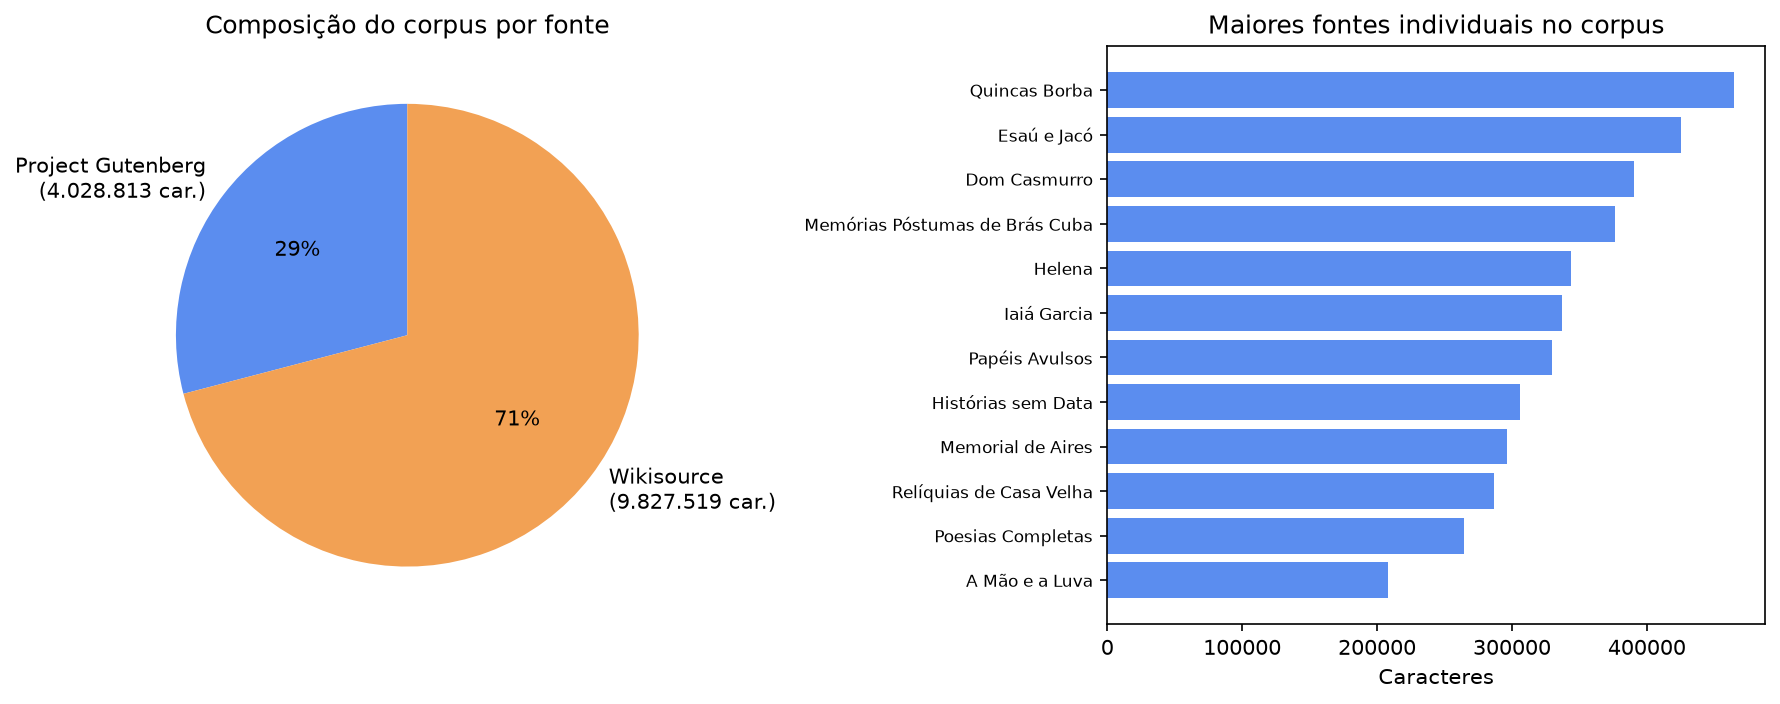
\includegraphics[width=\linewidth]{figuras/corpus_composicao.png}
\caption{Composição do corpus por fonte (esquerda) e maiores textos
individuais (direita), gerada automaticamente a partir do
\texttt{manifest.json} de proveniência.}
\label{fig:corpus}
\end{figure}

\section{Arquitetura e Configuração de Treino}
\label{sec:setup}

O modelo é um \textit{Transformer} decodificador-apenas no estilo GPT-2, na
configuração ``baby GPT'' padrão do próprio nanoGPT para \textit{datasets}
pequenos (Tabela~\ref{tab:arch}), totalizando 10.715.520 parâmetros ($\approx$
10,72M, com \textit{embedding} de entrada e cabeça de saída amarrados).

\textbf{Como se chega a esse número.} O \textit{embedding} de token contribui
$vocab\_size \times n_{embd} = 177 \times 384 = 67.968$ parâmetros. Cada um
dos 6 blocos \textit{Transformer} soma três partes: (i) atenção -- uma
projeção conjunta Q/K/V ($n_{embd} \rightarrow 3\,n_{embd}$, com viés) mais
uma projeção de saída ($n_{embd} \rightarrow n_{embd}$, com viés), totalizando
$(384{\times}1152 + 1152) + (384{\times}384 + 384) = 591.360$; (ii) MLP --
duas projeções ($n_{embd} \rightarrow 4\,n_{embd}$ e $4\,n_{embd}
\rightarrow n_{embd}$, ambas com viés), totalizando $(384{\times}1536 +
1536) + (1536{\times}384 + 384) = 1.181.568$; (iii) duas normalizações de
camada (\textit{LayerNorm}, peso + viés cada), $4 \times 384 = 1.536$. Um
bloco completo soma $591.360 + 1.181.568 + 1.536 = 1.774.464$ parâmetros;
seis blocos, $10.646.784$. Somando a \textit{LayerNorm} final ($768$) e o
\textit{embedding} de token ($67.968$) chega-se a $\mathbf{10.715.520}$.
Duas partes ficam de fora dessa soma: a cabeça de saída, porque seus pesos
são \emph{amarrados} (\textit{weight tying}) aos do \textit{embedding} de
token -- não é uma matriz extra, é a mesma reaproveitada --, e o
\textit{embedding} de posição ($block\_size \times n_{embd} = 256 \times
384 = 98.304$), excluído por convenção do próprio nanoGPT (sua função
\texttt{get\_num\_params}) por não representar capacidade de armazenar
conteúdo do texto, só de posição relativa dentro da janela de contexto.

\begin{table}[!t]
\centering
\caption{Hiperparâmetros do modelo e do otimizador (config. de referência)}
\label{tab:arch}
\begin{tabular}{@{}ll@{}}
\toprule
Hiperparâmetro & Valor \\
\midrule
Camadas ($n_{layer}$) & 6 \\
Cabeças de atenção ($n_{head}$) & 6 \\
Dimensão do \textit{embedding} ($n_{embd}$) & 384 \\
Contexto ($block\_size$) & 256 caracteres \\
\textit{Dropout} & 0,2 \\
Vocabulário (nível de caractere) & 177 \\
\textit{Batch size} & 128 \\
Otimizador & AdamW ($\beta_2=0{,}99$) \\
\textit{Learning rate} (máx.\ / mín.) & $10^{-3}$ / $10^{-4}$ \\
Cronograma de LR & \textit{warmup} (100) + cosseno \\
\bottomrule
\end{tabular}
\end{table}

\begin{figure}[!t]
\centering
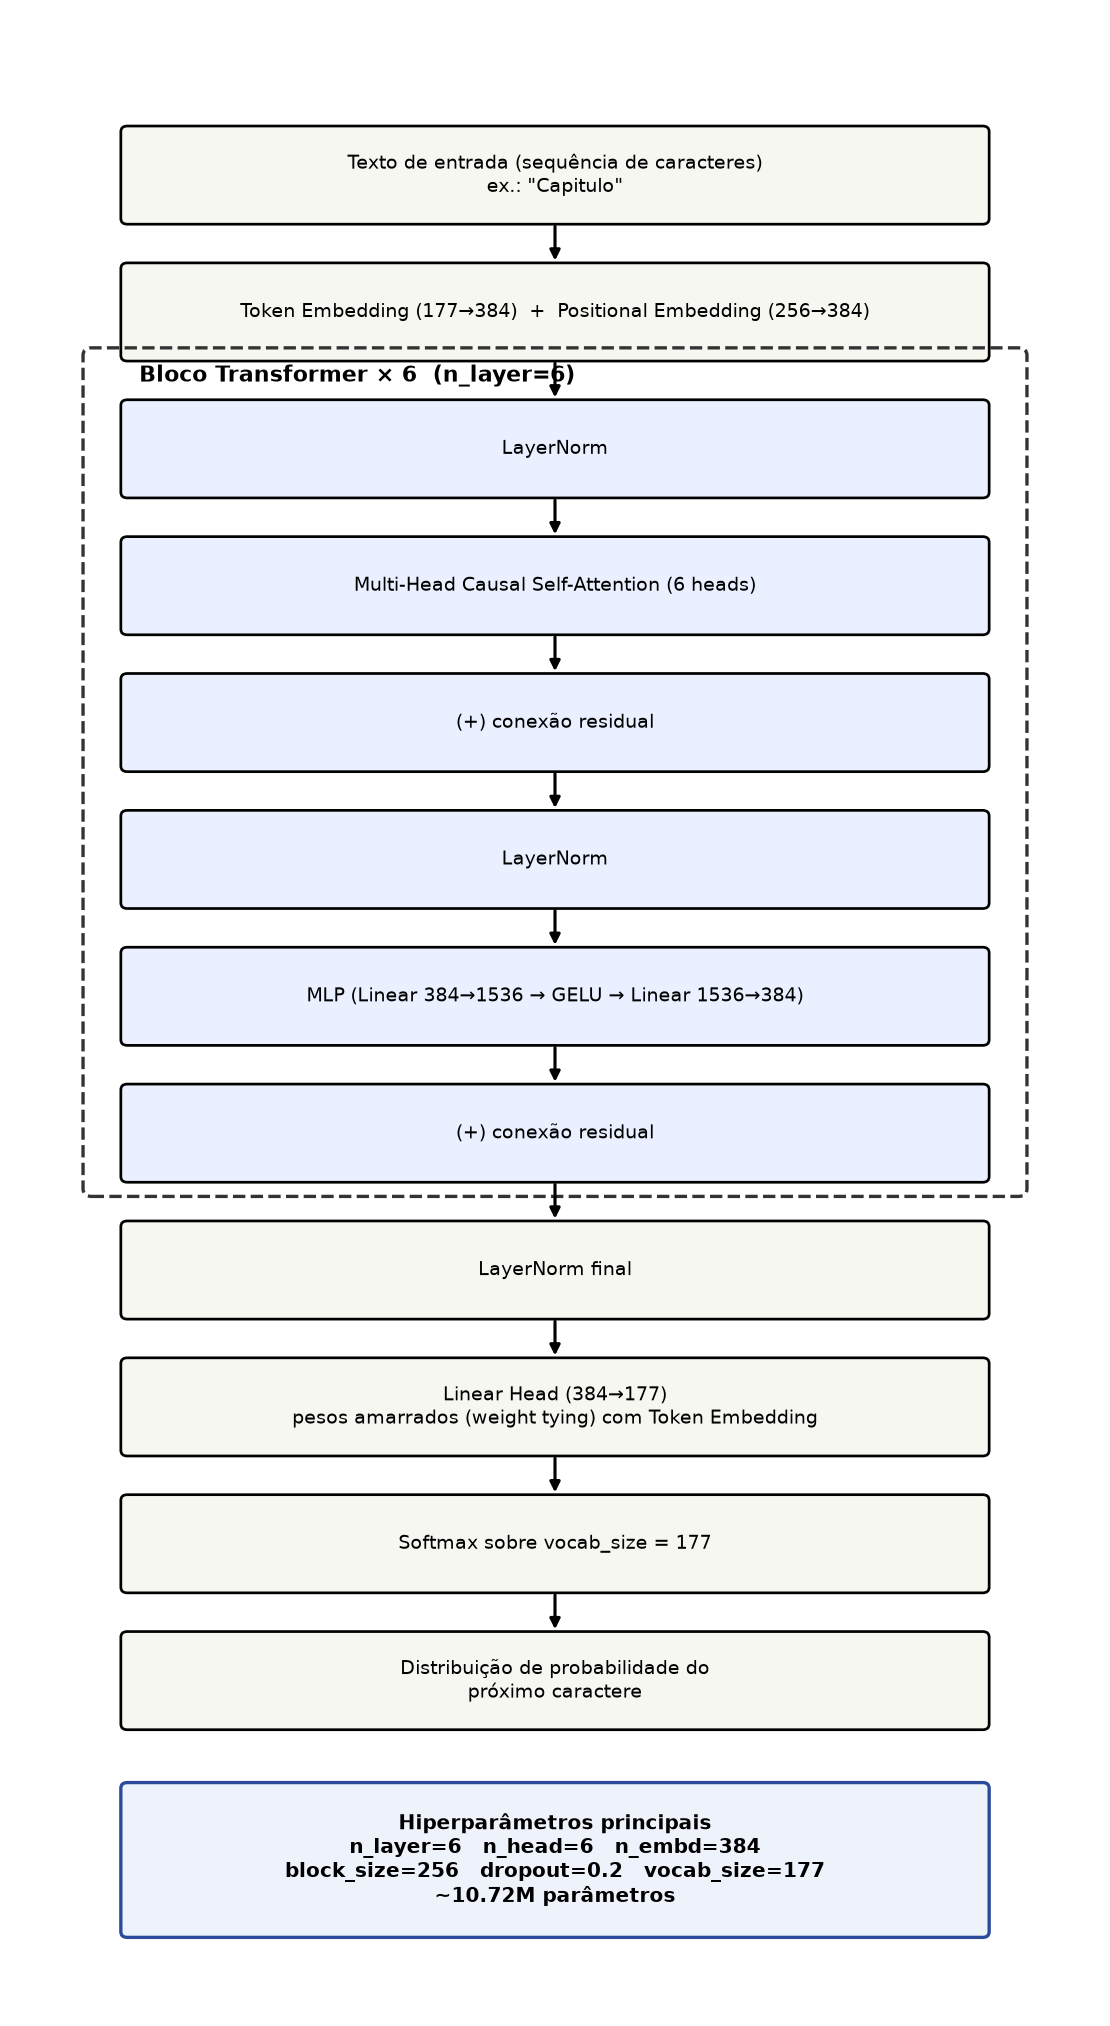
\includegraphics[width=\linewidth]{figuras/arquitetura_gpt.png}
\caption{Diagrama da arquitetura, gerado automaticamente a partir da própria
classe \texttt{GPT} do nanoGPT (contagem exata de parâmetros).}
\label{fig:arquitetura}
\end{figure}

\textbf{Portabilidade de \textit{hardware}.} O enunciado recomenda a entrega
via Google Colab, mas o desenvolvimento e boa parte dos treinos deste
trabalho ocorreram localmente, em um MacBook com Apple Silicon (backend MPS).
O \texttt{train.py} original do nanoGPT só reconhece \texttt{device\_type=
'cuda'} para fins de \textit{autocast}; fora do CUDA, ele cai silenciosamente
em precisão total (\textit{float32}), sem aproveitar precisão mista. Foi
aplicado um \textit{patch} mínimo (código próprio, documentado como tal no
notebook) que estende esse reconhecimento para \texttt{'mps'}, e foi
modernizada a chamada do \texttt{GradScaler} para a API atual do PyTorch
(\texttt{torch.amp}), sem alterar o comportamento em CUDA -- garantindo que o
mesmo notebook produza resultados comparáveis tanto no Colab quanto
localmente.

\section{Resultados Experimentais}
\label{sec:resultados}

\subsection{Efeito do corpus e do orçamento de treino}

Três rodadas completas isolam, uma de cada vez, o efeito do tamanho do
corpus e do número de iterações, mantendo a arquitetura da
Tabela~\ref{tab:arch} fixa (Tabela~\ref{tab:progressao}).

\begin{table}[!t]
\centering
\caption{Progressão dos resultados (val.\ loss e perplexidade)}
\label{tab:progressao}
\begin{tabular}{@{}lrrl@{}}
\toprule
Rodada & Corpus & Iters & Val.\ loss (perplex.) \\
\midrule
Baseline nanoGPT\footnotemark[1] & $\approx$1MB & 5000 & 1,4697 (4,35) \\
\textit{Resultados 1} & 4,0M car. & 5000 & 1,3345 (3,80)$^\dagger$ \\
\textit{Resultados 2} & 14,0M car. & 5000 & 1,2097 (3,35) \\
\textbf{\textit{Resultados 3}} & 14,0M car. & \textbf{15000} & \textbf{1,1040 (3,02)} \\
\bottomrule
\end{tabular}
\footnotetext[1]{\texttt{shakespeare\_char}, GPU A100 (número oficial do repositório).}
\footnotetext{$^\dagger$\textit{Overfitting} visível a partir da iteração $\approx$4000.}
\end{table}

\textit{Resultados 1} (só Gutenberg, 4,0M caracteres) já supera o baseline
oficial do nanoGPT, mas mostra \textit{overfitting} claro a partir da
iteração $\approx$4000 (a \textit{val loss} para de acompanhar a
\textit{train loss}). Ao maximizar o corpus (\textit{Resultados 2}), o mesmo
orçamento de 5000 iterações produz uma \textit{val loss} melhor
\emph{e sem overfitting} -- a curva de validação ainda caía na última
iteração, sugerindo que o modelo estava sub-treinado, não que havia
convergido. \textit{Resultados 3} confirma essa hipótese: estendendo o
orçamento para 15000 iterações com o mesmo corpus maximizado, a
\textit{val loss} continua caindo de forma consistente
(Figura~\ref{fig:loss}), terminando em 1,1040 (perplexidade $\approx 3{,}02$)
sem nenhum sinal de \textit{overfitting} -- o melhor resultado validado deste
trabalho. A taxa de melhoria, no entanto, desacelera visivelmente após a
iteração $\approx$10000, motivando a busca de melhorias adicionais na
Seção~\ref{sec:busca}.

\begin{figure}[!t]
\centering
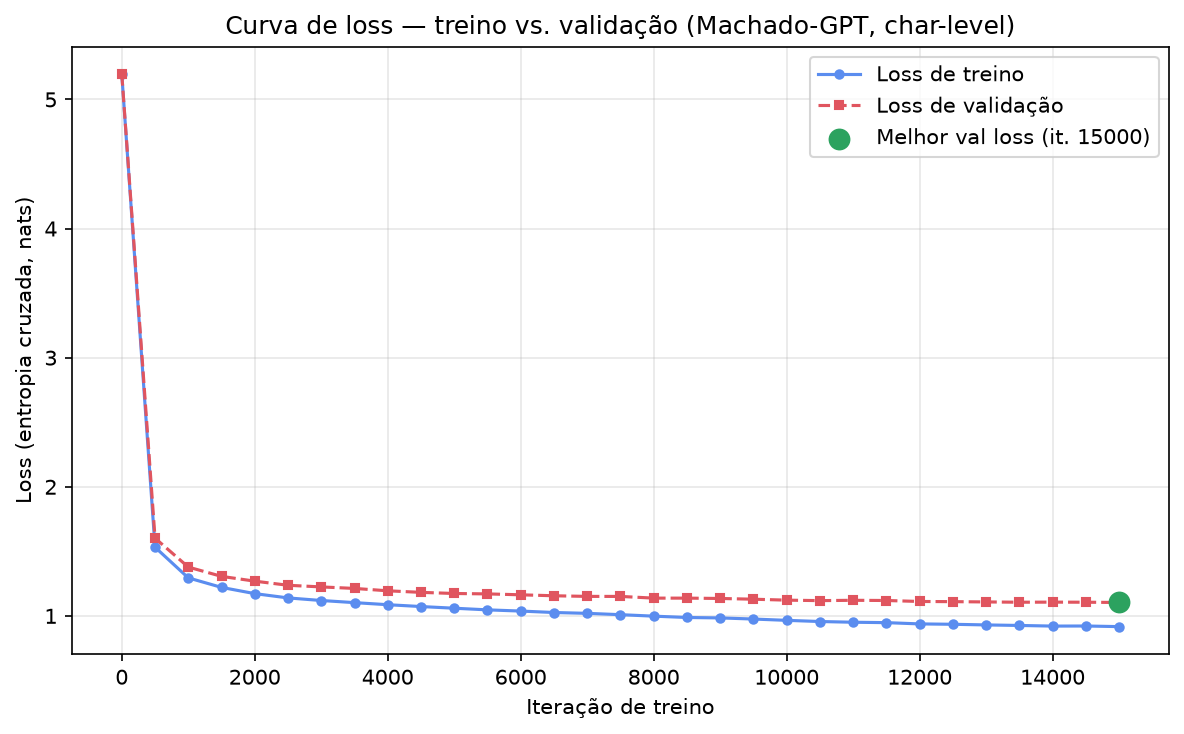
\includegraphics[width=\linewidth]{figuras/loss_curve.png}
\caption{Curva de \textit{loss} de treino/validação, \textit{Resultados 3}
(15000 iterações, corpus completo). Sem sinal de \textit{overfitting}.}
\label{fig:loss}
\end{figure}

\subsection{Avaliação qualitativa}

Amostras foram geradas com \texttt{sample.py} (\texttt{temperature=0.8},
\texttt{top\_k=200}), a partir do \textit{prompt} ``Capitulo'', usando o
\textit{checkpoint} de \textit{Resultados 3}. Um exemplo representativo:

\begin{quote}
\small\itshape
Capitulo III\\
Era falso da paixão acceita. Era a outra que Rita casára e riu dalli a pouco;
lá iriam commigo. Antes de me dizer não falar deste capitulo, voltaria
depois, e provavelmente falaria della com muita ternura e communicação.
Capitú, que o dissesse:\\
--Quanto a mim, estou muito bonita.
\end{quote}

Duas outras amostras, geradas com o mesmo \textit{prompt} e parâmetros,
ilustram a mesma mistura de acerto lexical e limitação estrutural:

\begin{quote}
\small\itshape
Capitulo. Os primeiros capitulos proprios disseram-me que eu lhe desse a
mesma mocidade, e que vingança entre a minha e da fidelidade. Não vinha a
casa de mana Rita, que estava passando na mesma semana.
\end{quote}

\begin{quote}
\small\itshape
A visita do cazamento era principalmente a minha mãe. Contei-lhe tudo o que
senti ainda na minha parte. Não me lembro se fora de semelhante
intervenção. Com effeito, á semelhança de acompanhar Emilia, fui ao
theatro [...]
\end{quote}

O modelo produz nomes de personagens reais e reconhecíveis (``Capitú'', de
\textit{Dom Casmurro}, com acentuação correta), diálogo bem formado
(travessão + fala curta) e mistura de ortografia de época e moderna
(``paixão'', ``della'', ``communicação''), consistente com as duas fontes do
corpus. Como esperado para um modelo em nível de caractere com contexto de
apenas 256 símbolos, a coerência é local (gramatical/estilística), sem
coerência narrativa de longo alcance.

\section{Busca Automatizada de Melhorias}
\label{sec:busca}

\subsection{Motivação e metodologia}

A desaceleração observada após a iteração $\approx$10000 em
\textit{Resultados 3} sugere que o gargalo deixou de ser o orçamento de
treino e passou a ser a combinação arquitetura/hiperparâmetros. Em vez de
ajustar manualmente, foi construída uma infraestrutura de busca com três eixos
independentes -- (A) arquitetura e hiperparâmetros, (B) \textit{embedding}
posicional, (C) tokenização -- avaliados por validação cruzada \textit{k-fold}
\textbf{por obra} (não por caractere): cada uma das 1.793 obras/páginas do
corpus é atribuída inteira a um de $k$ \textit{folds} por um algoritmo guloso
de \textit{bin-packing} (maior obra primeiro, sempre para o \textit{fold} com
menor total acumulado), evitando tanto o viés do corte contíguo 90/10 padrão
quanto o vazamento de contexto de um \textit{k-fold} ingênuo por caractere.

Para o eixo (A), foi usado \textit{successive halving} em três estágios (8
configurações $\rightarrow$ 4 $\rightarrow$ 2, com orçamento crescente de
600/1500/3000 iterações e 1/2/3 \textit{folds}), tratando arquitetura
($n_{layer}$, $n_{head}$, $n_{embd}$, \textit{block\_size}) como mais um
hiperparâmetro amostrado junto com \textit{dropout}/\textit{learning
rate}/\textit{batch size}. Para (B), foram comparadas quatro estratégias de
posição com arquitetura fixa: \textit{embedding} aprendido (padrão do GPT-2),
tabela senoidal fixa \cite{vaswani2017attention}, RoPE
\cite{su2021roformer} e ausência total de informação posicional. Para (C),
foi comparado o nível de caractere com um BPE próprio, treinado no corpus
(vocabulário de 1.500 \textit{tokens} -- pequeno de propósito, para não
desequilibrar o orçamento de parâmetros frente ao BPE completo do GPT-2, de
50.257 \textit{tokens}) \cite{sennrich2016bpe}; como \textit{tokens} de
granularidade diferente não são comparáveis por \textit{loss} bruta, foi usada
\textit{bits-por-caractere} (BPC) como métrica normalizada.

\subsection{Resultados da busca (orçamento curto)}

Os três eixos apontaram candidatos que batem a configuração de referência
(Tabela~\ref{tab:busca}), todos com margem grande o suficiente para não
serem ruído (foi verificado que os treinos de todas as variantes convergiram de
forma saudável nesse orçamento curto).

\begin{table}[!t]
\centering
\caption{Vencedores da busca por eixo (validação \textit{k-fold}, orçamento curto)}
\label{tab:busca}
\begin{tabular}{@{}llll@{}}
\toprule
Eixo & Candidato & Métrica & Baseline \\
\midrule
Arquitetura & 4/8/384/128\footnotemark[2] & 1,61 & 2,92 \\
Posição & RoPE & 2,76 & 3,07 (learned) \\
Tokenização & BPE (1500) & 3,59 BPC & 4,10 BPC (char) \\
\bottomrule
\end{tabular}
\footnotetext[2]{$n_{layer}/n_{head}/n_{embd}/block\_size$.}
\end{table}

\subsection{Confirmação em orçamento completo: os três falharam}
\label{sec:falha}

Como esses números vêm de um orçamento curto (3000 iterações) sobre um
\textit{split} mais difícil que o padrão, cada candidato foi replicado de forma
isolada em orçamento completo (15000 iterações, \textit{split} 90/10 padrão,
mesma metodologia de \textit{Resultados 1--3}). \textbf{Nenhum dos três se
confirmou} (Figura~\ref{fig:falha}, Tabela~\ref{tab:falha}): a arquitetura
candidata atinge um bom ponto na iteração $\approx$1500 (\textit{val loss}
1,56) e então sofre um salto abrupto para $\approx$3,15, onde permanece
travada pelo resto do treino; o BPE oscila sem nunca convergir de fato,
terminando pior do que em pontos intermediários; o RoPE diverge por completo
-- a \textit{loss} vira \texttt{NaN} de forma permanente a partir da
iteração $\approx$4200, desperdiçando 72\% do orçamento de treino restante.
Uma quarta variação, combinando os três candidatos, foi interrompida de
propósito após observar as três falhas isoladas.

\begin{table}[!t]
\centering
\caption{Confirmação em orçamento completo (15000 iters, \textit{split} padrão)}
\label{tab:falha}
\begin{tabular}{@{}llc@{}}
\toprule
Variação & Melhor \textit{val loss} (antes de falhar) & Diverge? \\
\midrule
Arquitetura & 1,56 (iter $\approx$1500) & Trava em $\approx$3,15 \\
RoPE & 2,63 (iter $\approx$2500) & \textbf{NaN} (iter $\approx$4200) \\
BPE (1500) & 4,40 (iter $\approx$2500) & Oscila, termina em 5,10 \\
\bottomrule
\end{tabular}
\end{table}

\begin{figure}[!t]
\centering
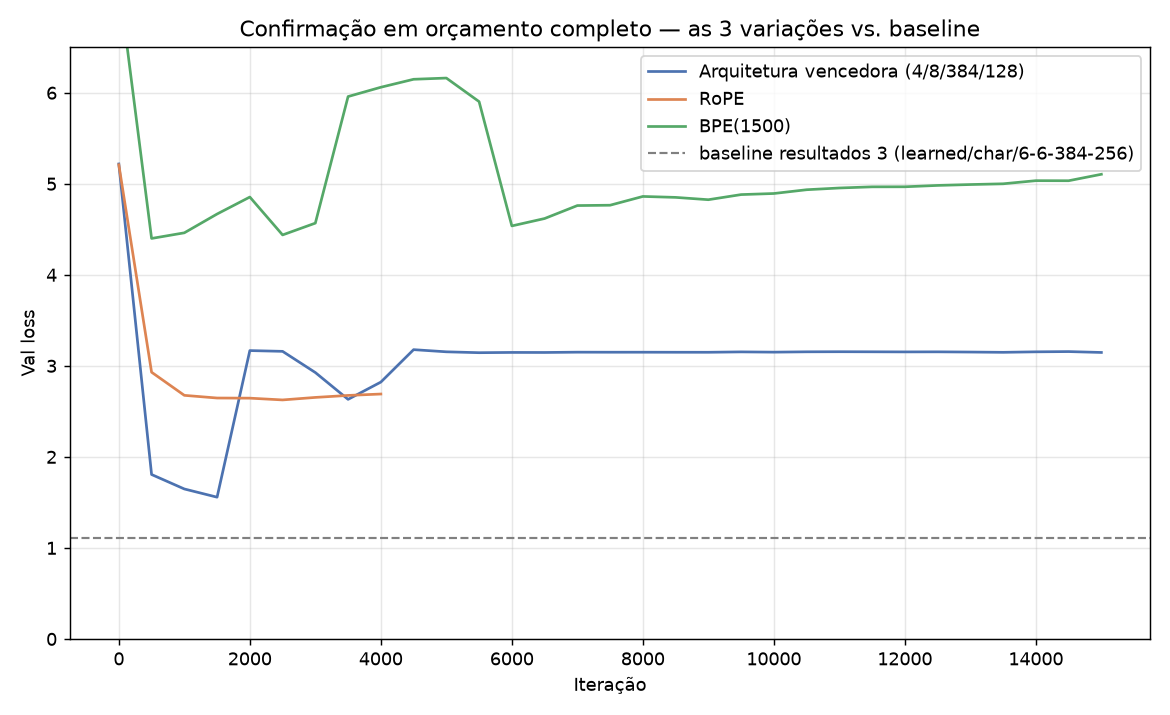
\includegraphics[width=\linewidth]{figuras/loss_curve_comparativo.png}
\caption{As três confirmações em orçamento completo, comparadas à referência
(\textit{Resultados 3}, linha tracejada). A curva do RoPE termina em
$\approx$4000 iterações porque, a partir daí, todos os valores são
\texttt{NaN}.}
\label{fig:falha}
\end{figure}

\textbf{Diagnóstico.} A causa mais provável é a ausência de um
\texttt{GradScaler} funcional sob \textit{autocast} de precisão mista
(\textit{float16}) no backend MPS: o \texttt{GradScaler} do PyTorch é
específico para CUDA e se torna um \textit{no-op} fora dele, deixando o
treino sem proteção contra gradientes grandes demais para \textit{float16}.
A referência (\textit{Resultados 3}) treinou 15000 iterações sem esse
problema, mas é a única combinação validada nesse orçamento longo; qualquer
uma das três mudanças altera a paisagem de gradientes o suficiente para, mais
cedo ou mais tarde, produzir uma atualização destrutiva sem essa proteção.
Isso não invalida os achados da busca em si -- os três candidatos continuam
promissores em orçamento curto -- apenas mostra que confirmá-los de forma
segura exige desligar a precisão mista (\textit{float32} puro) nas rodadas
de confirmação, o que fica como trabalho futuro. Este resultado é registrado
não como uma falha a esconder, mas como um achado metodológico genuíno sobre
os limites de se buscar hiperparâmetros em orçamento reduzido e treinar em
precisão mista sem a devida proteção numérica -- particularmente relevante
em \textit{hardware} de consumidor (MPS), onde esse tipo de infraestrutura de
segurança numérica, padrão em CUDA, simplesmente não existe.

\section{Extensão Proposta: Perguntas e Respostas no Universo Machadiano}
\label{sec:extensao}

O modelo treinado neste trabalho é puramente autorregressivo, sem qualquer
etapa de ajuste para seguir instruções -- ele completa texto no estilo de
Machado, mas não responde perguntas. Estendê-lo diretamente (por exemplo,
tentar fazer \textit{fine-tuning} supervisionado do próprio modelo de $\approx$
10,7M parâmetros em pares pergunta-resposta) provavelmente não funcionaria
bem: o contexto de 256 caracteres é curto demais para conter uma pergunta e
um trecho relevante de resposta, e o modelo é pequeno demais para desenvolver
capacidade de seguir instruções do zero com poucos exemplos de
\textit{fine-tuning}.

É proposta, em vez disso, uma arquitetura de \textbf{recuperação aumentada por
geração (RAG)}, que reaproveita diretamente o corpus e a infraestrutura já
construídos: (i) segmentar o corpus (Seção~\ref{sec:corpus}) em passagens
(parágrafo ou capítulo), indexadas por \textit{embeddings} de sentença; (ii)
dada uma pergunta do usuário sobre o universo machadiano (personagens, tramas,
temas), recuperar as passagens mais relevantes por similaridade vetorial;
(iii) usar um modelo de linguagem maior e já instruído (não o modelo treinado
do zero neste projeto, que carece de escala para isso) para sintetizar uma
resposta \emph{condicionada} nas passagens recuperadas, citando a obra de
origem. Essa abordagem tem duas vantagens sobre tentar estender o modelo
pequeno diretamente: (a) as respostas ficam ancoradas no texto real de
Machado, reduzindo alucinação, e (b) o corpus e o \textit{pipeline} de
limpeza já construídos (Seção~\ref{sec:corpus}) são reaproveitados
integralmente como base de conhecimento, sem precisar retreinar nada. Uma
alternativa mais custosa -- \textit{fine-tuning} supervisionado de um modelo
já pré-treinado e instruído sobre um conjunto de perguntas e respostas
curado manualmente sobre a obra -- fica registrada como possibilidade, mas
exigiria a criação de um \textit{dataset} de instrução que este projeto não
contempla. Nenhuma das duas abordagens foi implementada; ambas ficam como
trabalho futuro, conforme pedido no enunciado.

\section{Limitações}
\label{sec:limitacoes}

Quatro limitações merecem registro explícito. Primeiro, a tokenização em
nível de caractere do modelo de referência é ineficiente frente a
alternativas por \textit{subword}: a Seção~\ref{sec:busca}-B mostra que um
BPE pequeno treinado no próprio corpus reduz o custo de codificação em
$\approx$2 caracteres por \textit{token}, e supera o char-level em
\textit{bits-por-caractere} -- mas essa comparação foi feita em orçamento
curto (Seção~\ref{sec:falha}), então o ganho real em orçamento completo
ainda não está confirmado. Segundo, o contexto de 256 caracteres é curto
mesmo para os padrões de um modelo pequeno, limitando qualquer coerência a
poucas frases -- uma restrição arquitetural, não de treino, que só um
\textit{block\_size} maior (ou uma tokenização mais eficiente) resolveria.
Terceiro, cada configuração da busca da Seção~\ref{sec:busca} foi treinada
uma única vez por \textit{fold}; não foi medida a variância entre sementes
aleatórias diferentes, então parte do que se atribui a diferenças entre
configurações pode incluir ruído de inicialização, especialmente nas
diferenças mais estreitas da Tabela~\ref{tab:busca}. Quarto, como discutido
na Seção~\ref{sec:falha}, a infraestrutura de treino em precisão mista no
backend MPS carece da proteção numérica que o \texttt{GradScaler} oferece em
CUDA -- uma limitação de \textit{hardware}/biblioteca, não do método
proposto, mas que impede, por ora, confirmar com segurança os candidatos
encontrados pela busca.

\section{Conclusão}

Foi construído, a partir de fontes de domínio público, um corpus de 14,0M
caracteres da obra de Machado de Assis -- maior que alternativas públicas
equivalentes -- e foi treinado, com o \textit{nanoGPT} como base obrigatória,
um GPT-2 em nível de caractere que atinge \textit{val loss} de 1,1040
(perplexidade $\approx 3{,}02$) sem \textit{overfitting}, superando tanto o
baseline oficial do nanoGPT quanto as rodadas anteriores deste trabalho. Um
estudo controlado isolou o efeito do tamanho do corpus e do orçamento de
treino sobre esse resultado. Foi construída ainda uma infraestrutura de busca
automatizada (validação cruzada \textit{k-fold} por obra, \textit{successive
halving}) para três eixos de melhoria -- arquitetura, \textit{embedding}
posicional e tokenização --, cujos candidatos promissores em orçamento curto
falharam de forma sistemática ao serem confirmados em orçamento completo,
revelando e diagnosticando um limite real do treino em precisão mista no
backend MPS. Por fim, foi proposta uma extensão baseada em recuperação
aumentada por geração (RAG) para responder perguntas no universo machadiano,
reaproveitando o corpus e o \textit{pipeline} já construídos. Como trabalho
futuro, ficam: (i) confirmar os três candidatos da busca em precisão total
(\textit{float32}); (ii) implementar a extensão de RAG proposta na
Seção~\ref{sec:extensao}.

\section*{Código e Reprodutibilidade}

O código completo -- \textit{notebook} Google Colab autocontido, com
marcação explícita de trechos de terceiros, adaptados e próprios, além do
\textit{pipeline} de construção do corpus e da infraestrutura de busca
descrita na Seção~\ref{sec:busca} -- está disponível junto à entrega deste
projeto.

\bibliographystyle{IEEEtran}
\bibliography{referencias}

\end{document}
